\documentclass[11pt]{article}
\usepackage[utf8]{inputenc}
\usepackage{hyperref}
\usepackage{booktabs}
\usepackage{amssymb} % \nRightarrow
\usepackage{graphicx}
\usepackage{pifont} % \ding{51} = check, \ding{55} = cross

% =====================================================================================
% KLU-110 — Paper 3 SKELETON DRAFT. NOT FOR SUBMISSION.
% Thesis: aggregate detection-F1 masks failures on the rare, high-stakes tokens that carry
% re-identification. National IDs are the clearest provable case (deterministic, decode-bearing),
% not the whole of it.
%
% HARD CLAIM-DISCIPLINE GUARDS (do not relax without sign-off):
%   * Say "first UNIFIED", NEVER bare "first".
%   * "re-identification" is reserved for the DETERMINISTIC national-ID channel only.
%     The name/QI channels are "residual distinctiveness" / "name-in-context leak", NEVER re-id.
%   * Every number is config_status=dev: a FINDING, not yet validated/citable. SOTA / "best
%     protector" claims are GATED on KLU-27 (native-speaker + IAA) — see \sotagate.
%   * Re-run the prior-art rescan (KLU-15) before ANY broadened public claim.
%   * The name-in-context channel is PRELIMINARY / in-progress (KLU-118), NOT a cited headline:
%     its sample basis (split:test, 440/681 subjects) is not reconciled with the board's n=1123,
%     and it predates KLU-27. The QI-combination (PURR) metric is FUTURE WORK (KLU-122).
%   * No SOTA claims anywhere in this draft.
% =====================================================================================

% Reusable placeholder for the SOTA gate (KLU-27). Use wherever a "best/strongest/SOTA"
% statement would otherwise be tempting.
\newcommand{\sotagate}{\textbf{[SOTA-CLAIM GATED on KLU-27: native-speaker + inter-annotator
agreement sign-off on \texttt{ro-realskeleton} must clear the \texttt{dev} tracks before any
``best/strongest/SOTA'' wording. Re-run the KLU-15 prior-art rescan before broadening the public
claim, which predates the 3-ID / legal / Track-C expansion.]}}

\title{Detection Is Not Re-identification: A Unified Dissociation\\
       and an Open Protector for European De-identification\\
       \large (SKELETON DRAFT --- KLU-110 --- NOT FOR SUBMISSION)}
\author{KlusAI}
\date{2026}

\begin{document}
\maketitle

\begin{abstract}
% POSITIONING DISCIPLINE: "first UNIFIED", never bare "first". re-id reserved for the national-ID channel.
% All numbers config_status=dev, gated on KLU-27. No SOTA claims.
\noindent\textbf{Draft / skeleton --- not for submission.} High aggregate detection scores are the
standard way de-identification systems are reported and trusted. We show that this aggregate
\emph{masks} the failures that matter most: the rare, high-stakes tokens that actually carry
re-identification. Using the EuroPriv-Bench leaderboard~\cite{europrivbench2026}, we present the
first \emph{unified} demonstration that detection entity-F1 and re-identification protection are
\emph{dissociated} --- a high-F1 detector can still leak the decode-bearing national identifiers
(Romanian CNP, Polish PESEL, Italian Codice Fiscale) through which a subject is provably
re-identified. On the Romanian real-skeleton track, a strong general PII detector reaches entity-F1
$0.85$ yet leaks $30.2\%$ of distinct CNP subjects; a span-only spaCy baseline at F1 $0.14$ leaks
$89\%$; while an openly-released protector trained for the redaction objective leaks $0\%$ at F1
$0.74$. The dissociation holds across three national-ID schemes in three languages (RO/PL/IT) and
across two Romanian template families, and is statistically significant under an item-paired
McNemar test (e.g.\ $p\!=\!1.79\!\times\!10^{-102}$ vs.\ the F1 leader). We reserve the term
\emph{re-identification} for this deterministic national-ID channel. We separately report a
\textbf{preliminary, in-progress} second mechanism --- a name-in-context residual leak --- as
corroborating evidence of \emph{residual distinctiveness} (not re-identification), and frame the
quasi-identifier-combination metric as future work. We release the protector (kp-deid) and the
analysis harness. \sotagate{} All results are \texttt{config\_status=dev}: a finding, not yet a
validated or citable claim.
\end{abstract}

\section{Introduction}
\label{sec:intro}
% THESIS (one sentence): aggregate detection-F1 masks failures on the rare, high-stakes tokens that
% carry re-identification; national IDs are the clearest provable case, not the whole of it.
\textbf{Thesis.} \emph{Aggregate detection-F1 masks failures on the rare, high-stakes tokens that
carry re-identification: national IDs are the clearest provable case --- deterministic and
decode-bearing --- but not the whole of it.}

De-identification systems are routinely ranked by an aggregate detection metric (entity-level F1 or
recall). We argue this is the wrong target for a \emph{privacy} guarantee. A single missed
decode-bearing national identifier (e.g.\ a Romanian CNP, which encodes date of birth, sex, and
county of registration) re-identifies a subject regardless of how many low-stakes spans were caught.
Because such identifiers are rare relative to the token mass, a model can post a high aggregate F1
while still leaking them at a high rate.

This is, to our knowledge, the first \emph{unified} demonstration --- across three national-ID
schemes, three languages, and two template families, on one reproducible leaderboard --- that
detection accuracy and re-identification protection are \emph{dissociated} (we claim ``first
\emph{unified}'', not ``first'': the individual ingredients exist in prior art, but no prior artifact
combines them; Section~\ref{sec:related}, and re-verify via the KLU-15 rescan before any public
claim). We make the dissociation visual (a Pareto frontier, Figure~\ref{fig:pareto}), statistically
significant (item-paired McNemar), and actionable (an openly-released protector that escapes the
leak axis). \emph{Re-identification} is used \textbf{only} for the deterministic national-ID channel;
all other channels are framed as residual distinctiveness.

\paragraph{Contributions.}
\begin{enumerate}
  \item A unified \emph{detection $\neq$ re-identification} dissociation grounded in public
        leaderboard numbers across RO/PL/IT national-ID schemes and two RO template families
        (Section~\ref{sec:dissociation}).
  \item An item-paired significance test (McNemar) on per-subject national-ID protection, and a
        Pareto-frontier visualization of F1 vs.\ leak (Section~\ref{sec:dissociation},
        Figure~\ref{fig:pareto}).
  \item An openly-released protector (kp-deid) that sits \emph{off} the detection-optimal frontier:
        $0\%$ national-ID leak at non-maximal F1 (Section~\ref{sec:protector}).
  \item A \textbf{preliminary, in-progress} second mechanism (name-in-context residual leak) reported
        as corroborating evidence only, and a QI-combination metric stated as future work
        (Section~\ref{sec:corroborating}, Section~\ref{sec:futurework}).
\end{enumerate}

\section{Background and Threat Model}
\label{sec:threat}
% TODO: define decode-bearing national IDs (CNP/PESEL/Codice Fiscale), the per-subject
% (doc, country, normalized value) re-identification unit, and why a single leak re-identifies.
% Distinguish: (i) deterministic re-identification via a national ID; (ii) residual distinctiveness
% via names/QIs (NOT re-identification). State the GDPR Art. 4/9 framing (reuse the EuroPriv-Bench
% harmonized KP taxonomy~\cite{europrivbench2026}).
\textbf{[TODO]} Formalize the per-subject \emph{re-identification unit} $(\text{doc},
\text{country}, \text{normalized value})$ and the decode-bearing property of national IDs. Define
the \emph{leak rate} (fraction of distinct gold national-ID subjects left un-redacted on the
post-detection residual) and contrast it with detection F1. Reuse the EuroPriv-Bench harmonized
GDPR-aligned taxonomy~\cite{europrivbench2026} rather than re-deriving it.

\section{The Detection $\neq$ Re-identification Dissociation}
\label{sec:dissociation}
% PRIMARY EVIDENCE. All numbers from the EuroPriv-Bench leaderboard (ro/pl/it-realskeleton-v1),
% europriv_bench_version 0.2.0, taxonomy 0.2.0, config_status=dev. Source of truth:
% europriv-bench/baselines/leaderboard.json (ingested via `make results`).

\subsection{The headline anti-correlation (RO real-skeleton)}
On the Romanian real-skeleton track (\texttt{ro-realskeleton-v1}, $n{=}1123$ distinct CNP subjects),
detection F1 and CNP leak-rate move \emph{together}, not against each other, among content-NER
detectors. A strong general PII detector (GLiNER multi-pii) reaches entity-F1 $0.85$ yet leaks
$30.2\%$ of distinct CNP subjects; a span-only spaCy baseline at F1 $0.14$ leaks $89.0\%$; whereas
the kp-deid protector leaks $0\%$ at F1 $0.74$ --- it sits \emph{off} the detection-optimal frontier
(Figure~\ref{fig:pareto}, Table~\ref{tab:dissociation}). Higher detection accuracy did not buy
privacy protection.

\begin{figure}[t]
\centering
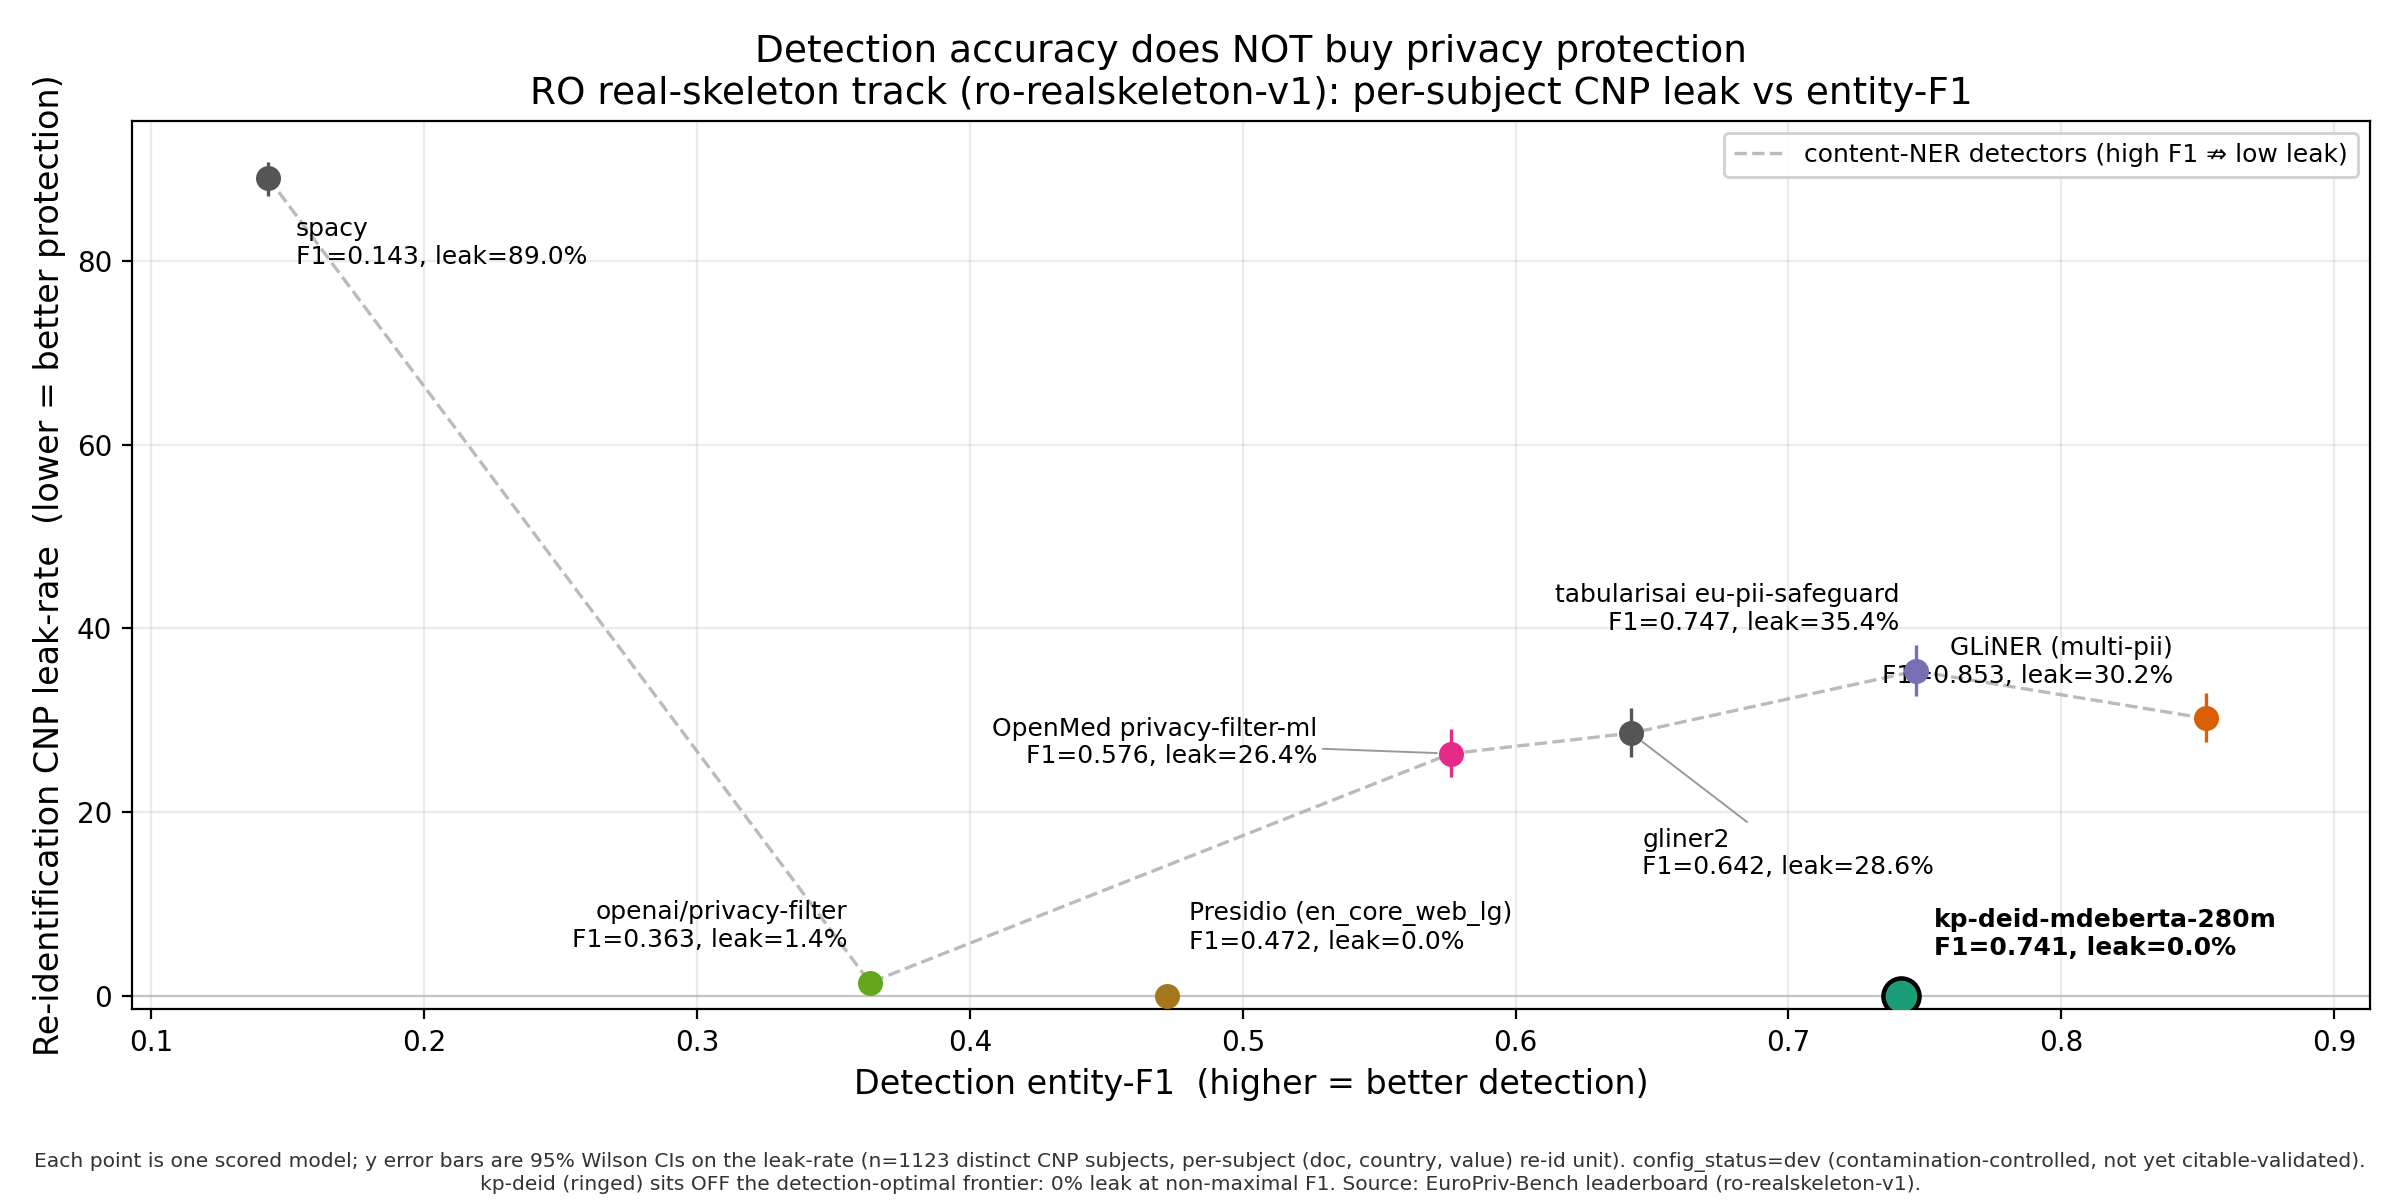
\includegraphics[width=\linewidth]{figures/pareto_dissociation_ro_realskeleton.png}
\caption{Detection accuracy does \emph{not} buy re-identification protection. Each point is one
scored model on \texttt{ro-realskeleton-v1}: detection entity-F1 ($x$) vs.\ per-subject CNP
re-identification leak-rate ($y$); $y$ error bars are $95\%$ Wilson CIs ($n{=}1123$ distinct CNP
subjects). Content-NER detectors lie on the dashed ``bad'' frontier (higher F1 $\nRightarrow$ lower
leak); kp-deid (ringed) sits off it at $0\%$ leak. \texttt{config\_status=dev}
(contamination-controlled, \textbf{not yet citable-validated}; gated on KLU-27). Figure regenerated
from the live leaderboard by \texttt{europriv-bench/analysis/pareto\_dissociation.py} (KLU-53) ---
no number is hardcoded.}
\label{fig:pareto}
\end{figure}

\begin{table}[t]
\centering
\small
\caption{Detection F1 vs.\ national-ID re-identification leak-rate across three national-ID schemes
in three languages (real-skeleton tracks). Leak-rate $=$ fraction of distinct gold national-ID
subjects left un-redacted. All entries \texttt{config\_status=dev}, \texttt{europriv\_bench} 0.2.0,
taxonomy 0.2.0. Source: EuroPriv-Bench leaderboard~\cite{europrivbench2026}
(\texttt{baselines/leaderboard.json}; ingested via \texttt{make results}). kp-deid (ours) is the only
system at $0\%$ leak on every track.}
\label{tab:dissociation}
\begin{tabular}{llcc}
\toprule
Track (ID scheme) & Model & Detection F1 & Re-id leak-rate \\
\midrule
RO (CNP)  & GLiNER multi-pii          & 0.85 & 30.2\% \\
RO (CNP)  & GLiNER2-base              & 0.64 & 28.6\% \\
RO (CNP)  & OpenMed privacy-filter-ml & 0.58 & 26.4\% \\
RO (CNP)  & spaCy \texttt{en\_core\_web\_lg} & 0.14 & 89.0\% \\
RO (CNP)  & \textbf{kp-deid (ours)}   & 0.74 & \textbf{0\%} \\
\midrule
PL (PESEL)& GLiNER multi-pii          & 0.82 & 57.8\% \\
PL (PESEL)& \textbf{kp-deid (ours)}   & 0.76 & \textbf{0\%} \\
\midrule
IT (Codice Fiscale) & GLiNER multi-pii & 0.86 & 36.2\% \\
IT (Codice Fiscale) & \textbf{kp-deid (ours)} & 0.70 & \textbf{0\%} \\
\bottomrule
\end{tabular}
\end{table}

\subsection{It holds across schemes, languages, and template families}
The dissociation is not a Romanian artifact. It reproduces on Polish PESEL (GLiNER F1 $0.82$,
leak $57.8\%$; kp-deid F1 $0.76$, leak $0\%$) and Italian Codice Fiscale (GLiNER F1 $0.86$, leak
$36.2\%$; kp-deid F1 $0.70$, leak $0\%$); see Table~\ref{tab:dissociation}. It also holds across two
independent Romanian template families (official correspondence; academic registry): a
difference-of-proportions test with Newcombe (1998) CIs shows the per-family gap CI excludes zero
for the typed content-NER detectors in both families (KLU-101 analysis artifact). This retires the
single-template-family caveat (KLU-114).
% TODO: ingest the per-family table from europriv-bench/analysis/family_dissociation_ro_realskeleton.md.

\subsection{Statistical significance (item-paired McNemar)}
We test per-subject national-ID protection with an item-paired McNemar test (each distinct gold
subject's national ID was either redacted or leaked; exact two-sided binomial $p$ on the discordant
pairs). On \texttt{ro-realskeleton-v1}, kp-deid vs.\ the F1 leader (GLiNER) gives discordant counts
$b{=}339$, $c{=}0$ ($p\!=\!1.79\!\times\!10^{-102}$): kp-deid protects subjects GLiNER leaks, never
the reverse. kp-deid vs.\ privacy-filter gives $b{=}16$, $c{=}0$ ($p\!=\!3.05\!\times\!10^{-5}$).
A genuine tie is reported honestly: kp-deid vs.\ Presidio gives $b{=}c{=}0$, $p{=}1$ (both reach
$0\%$ CNP leak on this track). Source: \texttt{analysis/mcnemar\_ro\_realskeleton.md} (KLU-53).

\section{An Open Protector that Escapes the Leak Axis}
\label{sec:protector}
% kp-deid-mdeberta-280m: trained for the redaction objective; 0% national-ID leak on RO/PL/IT
% real-skeleton at non-maximal but competitive F1. Openly released. Reproducible via the leaderboard
% submission protocol (SUBMISSIONS.md). NO "best protector" / SOTA wording here — gated.
We release \texttt{kp-deid-mdeberta-280m}, a $280$M-parameter protector trained for the redaction
objective rather than for span detection. It attains $0\%$ national-ID leak on all three
real-skeleton tracks (RO/PL/IT) at competitive but non-maximal detection F1 (Table~\ref{tab:dissociation}),
i.e.\ it sits off the detection-optimal frontier. The model and the scoring harness are openly
released; results are reproduced by CI through the public submission protocol, never self-reported.
\sotagate{}
% TODO: model card link, training-data provenance (synthetic train kept separate from held-out gold),
% architecture details, and the kp-deid v2 multilingual training note once that artifact lands.

\section{Corroborating Evidence: A Second, Independent Mechanism (Preliminary)}
\label{sec:corroborating}
% PRELIMINARY / IN-PROGRESS (KLU-118). NOT a cited headline. NOT re-identification.
% Sample basis (split:test, 440 ID-subjects / 681 name-subjects) is NOT yet reconciled with the
% board's n=1123, and predates KLU-27. Term: "name-in-context leak" / "residual distinctiveness".
\textbf{Preliminary / in-progress --- corroborating only; not a headline result and not yet
reconciled with the board.} Beyond the deterministic national-ID channel, an early analysis (KLU-118)
measures a second, \emph{independent} channel: a \texttt{PERSON} full name left un-redacted on the
post-detection residual --- a \emph{name-in-context leak}, i.e.\ \emph{residual distinctiveness}, which
we explicitly do \textbf{not} call re-identification. On \texttt{ro-realskeleton-v1}, Presidio leaks
$0\%$ of national IDs but $\sim\!13.7\%$ of names; spaCy shows the inverse profile (high ID leak,
low name leak); kp-deid leaks $0\%$ on both. A per-document $2\times2$ cross-tab indicates the two
channels are largely independent --- different systems fail on different channels --- which is why an
aggregate detection score hides both.

\textbf{Why this is not yet citable.} The name channel's sample basis (\texttt{split:test};
$440$ national-ID subjects and $681$ name subjects) is \emph{not yet reconciled} with the
$n{=}1123$ used for the board-grounded national-ID numbers, and the analysis predates the KLU-27
validation. We therefore present it as corroboration of the \emph{shape} of the dissociation, not as
a measured headline number.
% TODO: reconcile sample basis with n=1123; re-run post-KLU-27; ingest the reconciled cross-tab.

\section{Related Work}
\label{sec:related}
% Position against TAB, AI4Privacy, MAPA, MultiGraSCCo, MEDDOCAN, GLiNER2-PII, SPY; cite the
% concurrent RAT-Bench HONESTLY (complementary, U.S. demographics, no legal text, no GDPR taxonomy).
% Re-run the KLU-15 prior-art rescan before any broadened public claim (predates 3-ID/legal/Track-C).
This paper builds on the EuroPriv-Bench benchmark and leaderboard~\cite{europrivbench2026}, which
itself subsumes the prior de-identification art (TAB~\cite{pilan2022tab},
AI4Privacy~\cite{ai4privacy_openpii}, MAPA~\cite{mapa_toolkit},
MultiGraSCCo~\cite{multigrascco2026}, MEDDOCAN~\cite{meddocan2019},
GLiNER2-PII~\cite{gliner2pii2026}, SPY~\cite{spy2025}). Our contribution is orthogonal to the
benchmark: a \emph{unified dissociation} result and an open protector. The closest concurrent and
independent work is RAT-Bench~\cite{ratbench2026}, a hosted re-identification-risk leaderboard; it is
complementary rather than overlapping --- it is built on U.S.\ demographics
(English/Spanish/Chinese), contains no legal text, and uses no GDPR-aligned taxonomy, so it does not
address the European national-ID re-identification setting studied here.
\textbf{[TODO: re-run the KLU-15 prior-art rescan before any broadened public claim --- KLU-15
predates the 3-ID / legal / Track-C expansion. Confirm ``first \emph{unified}'' still holds and cite
any new concurrent dissociation work, e.g.\ RAT-Bench, honestly.]}

\section{Limitations}
\label{sec:limitations}
% Be honest. This is a finding, not a validated/citable claim.
\begin{itemize}
  \item \textbf{Not yet validated (\texttt{config\_status=dev}).} Every number here is a finding on
        contamination-controlled but \texttt{dev}-status tracks. SOTA / ``best protector'' claims are
        \textbf{gated on KLU-27} (native-speaker review + inter-annotator agreement on
        \texttt{ro-realskeleton}). \sotagate{}
  \item \textbf{Synthetic real-skeleton data.} The real-skeleton tracks are synthetic; the leak-rate
        measures protection on synthetic subjects, not a population re-identification rate against a
        real reference population.
  \item \textbf{Name-in-context channel is preliminary.} Its sample basis is not reconciled with the
        board's $n{=}1123$ and it predates KLU-27 (Section~\ref{sec:corroborating}).
  \item \textbf{No QI-combination metric yet.} We do not yet measure $k$-anonymity-style
        re-identification from \emph{combinations} of quasi-identifiers (the gold lacks binned QI
        tagging); see future work.
  \item \textbf{Prior-art recency.} The ``first \emph{unified}'' positioning must be re-verified
        against KLU-15 before any public claim.
\end{itemize}

\section{Future Work}
\label{sec:futurework}
% QI-combination (PURR) metric = KLU-122. Reconcile name channel. kp-deid v2 multilingual. KLU-27.
\begin{itemize}
  \item \textbf{QI-combination re-identification (PURR) metric (KLU-122).} Tag binned
        quasi-identifier tuples in gold (DOB/age band, sex, locality/NUTS, nationality, profession,
        rare-condition flag) to enable a $k$-anonymity-violation diagnostic --- moving from
        \emph{residual distinctiveness} toward measured population re-identification risk.
  \item \textbf{Reconcile and validate the name-in-context channel} against $n{=}1123$ post-KLU-27.
  \item \textbf{kp-deid v2 multilingual protector} and broadened track coverage.
  \item \textbf{Native-speaker + IAA validation (KLU-27)} to clear the \texttt{dev} tracks and unlock
        citable claims.
\end{itemize}

\bibliographystyle{plain}
\bibliography{../../shared/klusai}

\end{document}
